\appendix
\setcounter{figure}{0}
\renewcommand{\thefigure}{A\arabic{figure}}
\providecommand{\theHfigure}{}
\renewcommand{\theHfigure}{A\arabic{figure}}
\setcounter{table}{0}
\renewcommand{\thetable}{S\arabic{table}}
\providecommand{\theHtable}{}
\renewcommand{\theHtable}{S\arabic{table}}

\section{Common-Scale Model Profiles}
\label{app:patient-profiles}

Table~\ref{tab:patient-profiles} reports the exact model-level common-scale AUC estimates and paired patient-cluster confidence intervals underlying the visual comparison in Figure~\ref{fig:profile-forest}.

\begin{table*}[!t]
  \centering
  \small
  \caption{Common-five-scale model profiles with paired patient-cluster 95\% intervals. The semantic column reports the train-selected single-coordinate $|r|$ AUC defined in Section~\ref{sec:benchmark-design}. Each AUC integrates the same $E\in\{1,4,8,16,32\}$ support and averages the same five depth targets and three SAE seeds.}
  \label{tab:patient-profiles}
  \InputIfFileExists{generated/paper_table_multiscale_patient.tex}{}{%
    \fbox{\parbox{0.86\textwidth}{\centering Audited patient-profile table pending.}}%
  }
\end{table*}

\FloatBarrier
\section{Fixed-Scale Accessibility Calibration}
\label{app:accessibility-calibration}

Table~\ref{tab:accessibility-calibration} reports the complete held-out calibration that compares distributed ridge readouts with increasingly localized SAE, native-coordinate, and random-coordinate readouts at the common $E=8$ scale.

\begin{table*}[!b]
  \centering
  \small
  \setlength{\tabcolsep}{3pt}
  \caption{Held-out $E=8$ accessibility calibration over five depths and 49 concepts. Ridge columns report mean $|r|$. One-dimensional entries report mean $|r|$/coverage at $|r|\geq.20$; SAE values average three seeds and random values average 20 dictionaries. All coordinates are selected on training data only.}
  \label{tab:accessibility-calibration}
  \InputIfFileExists{generated/paper_table_accessibility_calibration.tex}{}{%
    \fbox{\parbox{0.86\textwidth}{\centering Audited accessibility-calibration table pending.}}%
  }
\end{table*}

\clearpage
\section{Frozen Source-Layer Interfaces}
\label{app:model-interfaces}

Table~\ref{tab:multiscale-models} defines the representation-extraction contract used throughout the benchmark. Each released checkpoint is frozen and evaluated through its native lead selection, temporal resolution, and tokenization path. The models consequently receive inputs ranging from eight to twelve leads and from 2,250 to 5,000 samples, while the audited states are taken before any model-specific downstream projection that would change the source width. Preserving these interfaces measures the representations available under realistic model use rather than introducing an untrained common tokenizer.

\begin{table*}[!t]
\centering
\small
\caption{Frozen source-layer interfaces. The benchmark preserves each released ECG input path while matching the analyzed layer width. ``Layers'' counts available audited states, including the indexed boundary states used by the released extraction code.}
\label{tab:multiscale-models}
\begin{tabular}{@{}lp{3.0cm}p{3.0cm}p{4.2cm}cc@{}}
\toprule
\textbf{Model} & \textbf{Pretraining family} & \textbf{Input used} & \textbf{Audited layer state} & \textbf{Layers} & $\boldsymbol{d}$ \\
\midrule
CSFM & multimodal sensing & $12\times2500$ & released encoder/classification stream & 6 & \textbf{768} \\
CARDIAC-FM & ECG+MRI risk & $12\times5000$ & transformer state before 768-to-512 pool projection & \textbf{12} & \textbf{768} \\
ECG-FM & wav2vec and contrastive & $12\times5000$ & token states & \textbf{12} & \textbf{768} \\
ECG-JEPA & joint-embedding prediction & $8\times2500$ & encoder states after released lead selection & \textbf{12} & \textbf{768} \\
HuBERT-ECG & masked clustering & flattened $12\times2500$ & token states & \textbf{12} & \textbf{768} \\
ST-MEM & spatio-temporal masking & $12\times2250$ & \texttt{forward\_encoding} states & \textbf{12} & \textbf{768} \\
\bottomrule
\end{tabular}
\end{table*}

The shared audited width $d=768$ permits exact capacity matching: the five expansion factors correspond to absolute dictionary widths $N\in\{768,3072,6144,12288,24576\}$, with the primary active budget fixed at $k=96$. Relative depth maps the six available CSFM states and the twelve states exposed by each other encoder onto the same five index positions, providing a common coordinate over each encoder trajectory. Table~\ref{tab:multiscale-models} specifies the resulting representation interfaces, and Appendix~\ref{app:input-harmonization} tests how heterogeneous waveform interfaces affect the final-layer model ordering.

\FloatBarrier
\section{Additional Depth--Scale Atlases}
\label{app:additional-atlases}

Figures~\ref{fig:reconstruction-atlas} and~\ref{fig:dead-feature-atlas} expose the two validation fidelity diagnostics for all 150 model--depth--scale configurations underlying the 450 trained SAE cells. Each heatmap cell averages the three fixed SAE seeds, and each metric uses one shared color scale across all six models. These complete surfaces complement the clinical-accessibility atlas in Figure~\ref{fig:semantic-atlas} and prevent a favorable depth or dictionary width from being selected in isolation.

\begin{figure*}[!t]
  \centering
  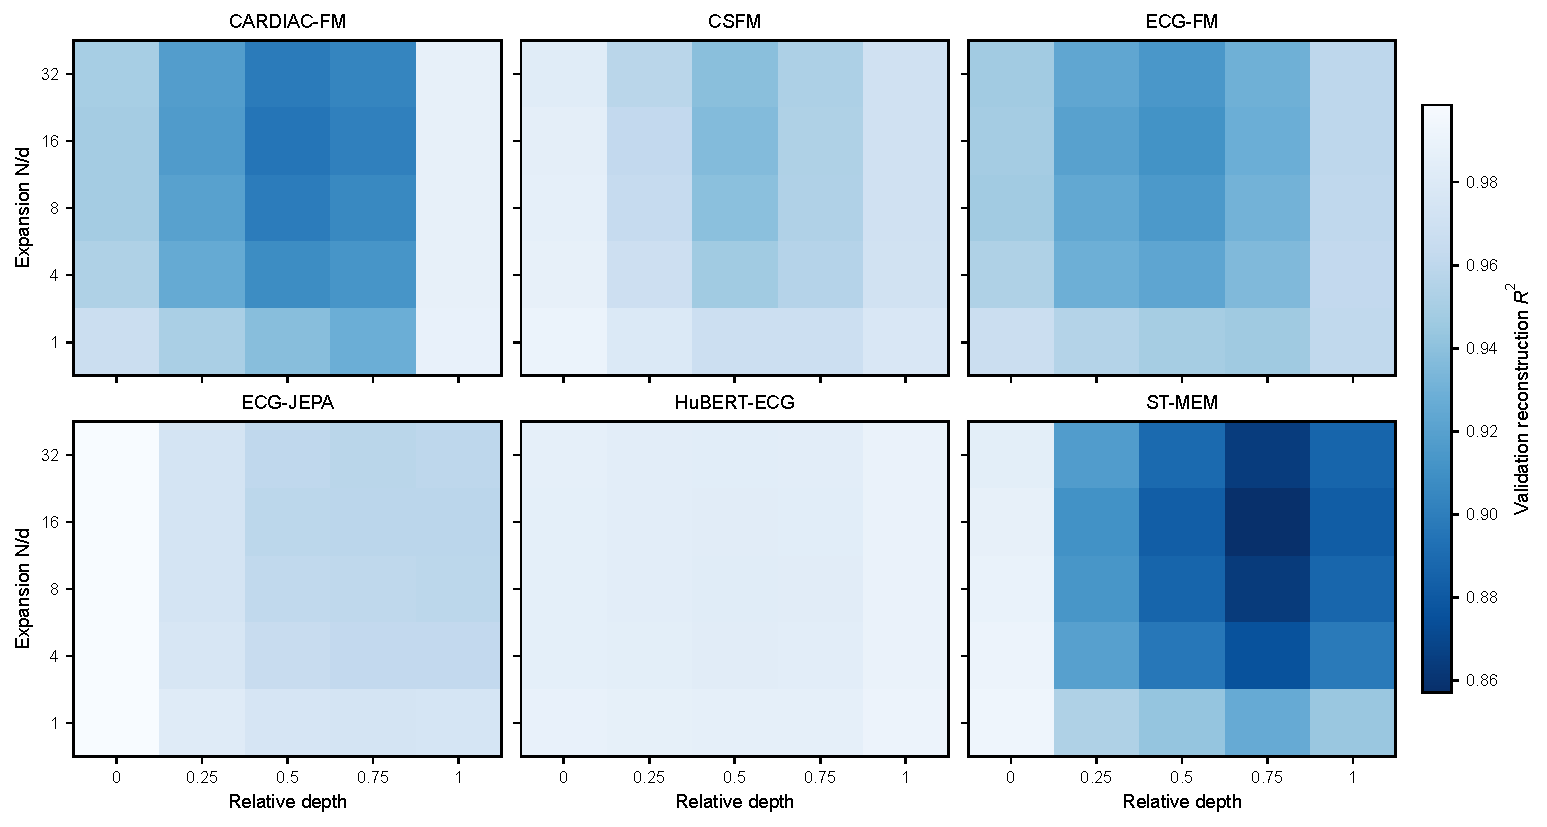
\includegraphics[width=\textwidth]{figures/multiscale_reconstruction_atlas.pdf}
  \caption{Validation reconstruction $R^2$ over the complete matched depth--scale atlas.}
  \label{fig:reconstruction-atlas}
  \Description{Six heatmaps show sparse-autoencoder reconstruction over five relative depths and five exactly matched expansion factors.}
\end{figure*}

Reconstruction remains high overall but does not improve monotonically with dictionary width under the fixed $k=96$ budget. Averaged descriptively over all models, depths, and seeds, validation $R^2$ is 0.968, 0.953, 0.949, 0.947, and 0.948 for $E=1,4,8,16,$ and 32, respectively. The model-averaged profiles range from 0.918 for ST-MEM to 0.986 for HuBERT-ECG, while the depth average falls from 0.978 at the initial state to approximately 0.937 at relative depths 0.5--0.75 before reaching 0.962 at the final state. Thus additional dictionary coordinates do not substitute for model- and depth-specific reconstruction structure when the active-code budget is held constant.

\begin{figure*}[!t]
  \centering
  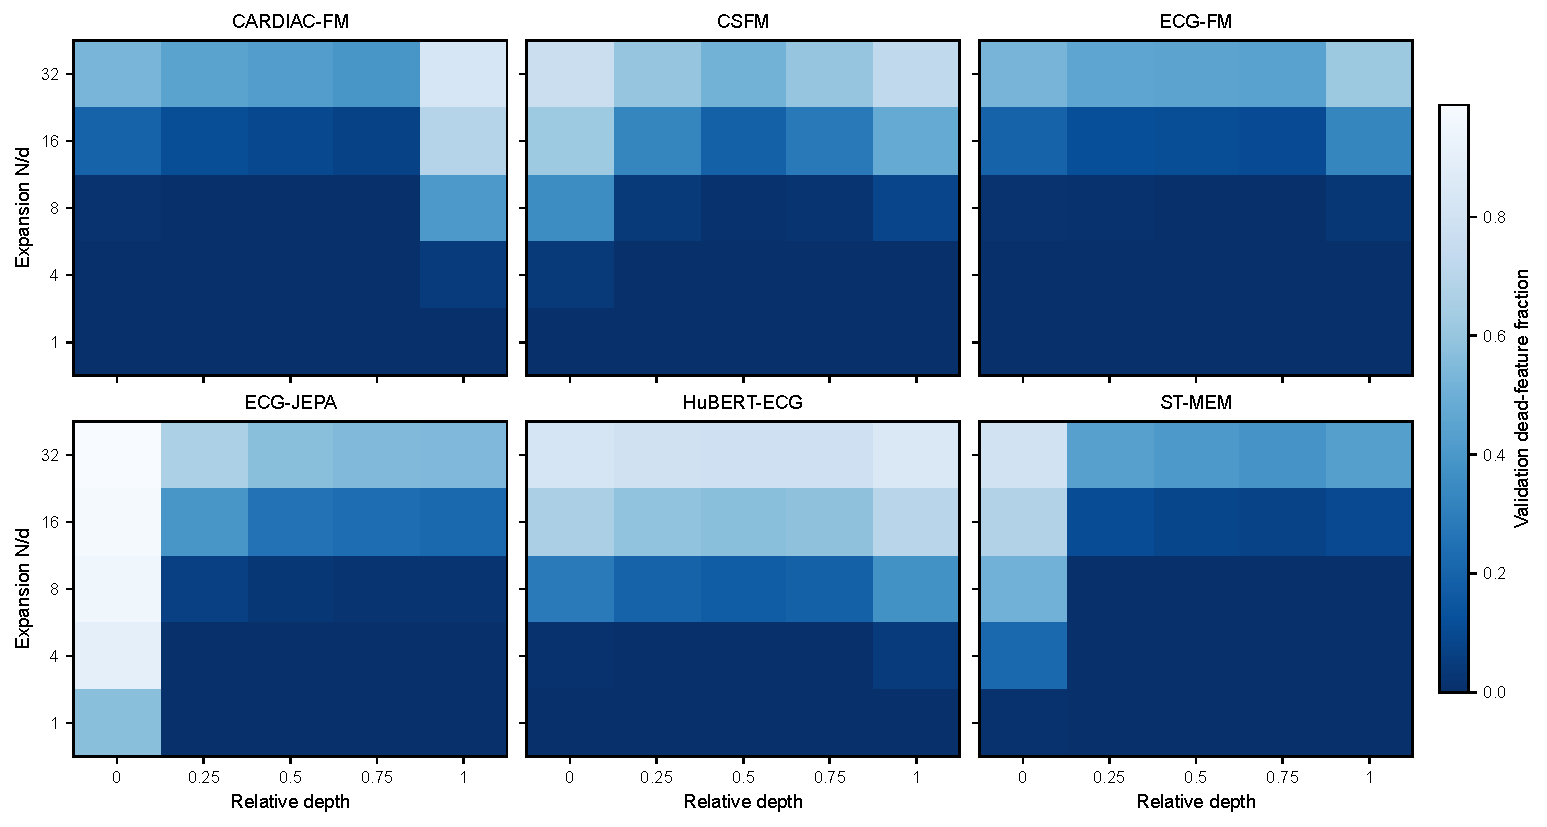
\includegraphics[width=\textwidth]{figures/multiscale_dead_feature_atlas.pdf}
  \caption{Validation dead-feature fraction over the complete matched depth--scale atlas.}
  \label{fig:dead-feature-atlas}
  \Description{Six heatmaps show dead-feature fractions over five relative depths and five exactly matched expansion factors.}
\end{figure*}

Dictionary utilization changes much more strongly with scale. The corresponding mean dead-feature fractions are 0.019, 0.042, 0.127, 0.338, and 0.604 from $E=1$ through $E=32$. Model-level averages range from 0.137 for ECG-FM to 0.337 for HuBERT-ECG, and the initial-state average (0.388) is substantially higher than the averages near relative depths 0.5 and 0.75 (0.156 and 0.158). HuBERT-ECG therefore combines the highest descriptive reconstruction average with the highest dead-feature average, directly illustrating that sparse fidelity and dictionary utilization are distinct properties. Reconstruction, dead-feature fraction, and the preregistered validation fidelity gate jointly characterize operating points across the complete dictionary-width curve.

\FloatBarrier
\section{Credentialed MIMIC-IV-ECG Replication}
\label{app:mimic-replication}

We repeated the multiscale SAE audit on the credentialed MIMIC-IV-ECG cohort~\cite{gow2023mimic}. The fixed manifest contains 100,000 ECGs from 48,491 patients, partitioned by patient into 70,260 training, 9,768 validation, and 19,972 test records; 54,591 records have complete waveform-derived measurements. Source waveforms and identifiers remain in the credentialed environment. The replication uses the same six frozen encoders, relative depths $\{0,.25,.5,.75,1\}$, expansion factors $E\in\{1,4,8,16,32\}$, $k=96$, three SAE seeds, and 8,000 training steps as the primary benchmark, for 450 completed SAE cells. For this SAE-only analysis, semantic alignment and coverage use seven continuous waveform concepts: heart rate, QRS duration, PR interval, a QT-like interval, and global R-, ST-, and T-amplitude measurements.

The model-level held-out profiles are reported in Table~\ref{tab:mimic-model-profiles}; this appendix provides the cohort, uncertainty, and scale--depth sensitivity details.

Patient-cluster uncertainty uses 2,000 test-set bootstrap draws over 6,609 patients, retaining all ECGs from each sampled patient. The leading profiles are precise: HuBERT-ECG reconstruction is 0.9905 (95\% CI 0.9904--0.9906), while ECG-JEPA semantic alignment is 0.3244 (0.3190--0.3299) and coverage is 0.7810 (0.7400--0.8057). The intervals quantify patient-sampling uncertainty conditional on the frozen encoders, trained SAEs, and training-selected coordinates.

The aggregate sensitivity analysis in Table~\ref{tab:mimic-scale-depth} demonstrates the resolution gained from a multiscale, multidepth audit. Across expansion factors, reconstruction remains near 0.97, semantic alignment is highest at $E=1$, and the dead-feature fraction traces dictionary utilization from 0.032 at $E=1$ to 0.636 at $E=32$. Across depth, semantic alignment is highest near relative depth 0.5 and coverage peaks near 0.75. These profiles show how MIMIC representation properties vary jointly with SAE capacity and encoder depth.

\begin{table*}[t]
  \centering
  \small
  \caption{MIMIC-IV-ECG scale and depth sensitivity, aggregated across the six models. Expansion rows average over five depths; depth rows average over five expansions. All rows average the three SAE seeds.}
  \label{tab:mimic-scale-depth}
  \begin{tabular}{llrrrr}
    \toprule
    Axis & Setting & Recon. $R^2$ & Semantic alignment & Coverage & Dead fraction \\
    \midrule
    Expansion & $E=1$  & 0.973 & \textbf{0.299} & \textbf{0.710} & 0.032 \\
              & $E=4$  & 0.971 & 0.281 & 0.624 & 0.134 \\
              & $E=8$  & 0.971 & 0.284 & 0.632 & 0.277 \\
              & $E=16$ & 0.971 & 0.284 & 0.637 & 0.461 \\
              & $E=32$ & 0.970 & 0.283 & 0.627 & \textbf{0.636} \\
    \midrule
    Relative depth & 0    & \textbf{0.986} & 0.295 & 0.640 & 0.542 \\
                   & 0.25 & 0.973 & 0.297 & 0.662 & 0.293 \\
                   & 0.50 & 0.964 & 0.298 & 0.689 & 0.211 \\
                   & 0.75 & 0.959 & 0.289 & 0.692 & 0.194 \\
                   & 1.00 & 0.973 & 0.252 & 0.546 & 0.301 \\
    \bottomrule
  \end{tabular}
\end{table*}

Matched decoder features vary across seeds (model-level stability AUC 0.293--0.378), whereas their selected subspaces are more reproducible (overlap AUC 0.702--0.778). This distinction identifies the selected subspace as the more stable unit for cross-seed interpretation and supports model-level conclusions about reproducible representation structure. The release audit passes all requirements with 450/450 SAE cells and no missing matched depth--scale block. Together, these results provide a complete credentialed-cohort replication of the benchmark profile.

\section{Input-Interface Harmonization Audit}
\label{app:input-harmonization}

The primary benchmark preserves each released model's input interface to reflect realistic use, but this choice could confound encoder differences with lead selection, sampling, or windowing. We therefore repeated final-layer dense-coordinate accessibility under four protocols on the same 21,799 PTB-XL records and patient split. \emph{Native} retains each released interface. \emph{Lead} supplies the common independent leads I, II, and V1--V6 and reconstructs the dependent limb leads for 12-lead models using
$\mathrm{III}=\mathrm{II}-\mathrm{I}$,
$\mathrm{aVR}=-(\mathrm{I}+\mathrm{II})/2$,
$\mathrm{aVL}=\mathrm{I}-\mathrm{II}/2$, and
$\mathrm{aVF}=\mathrm{II}-\mathrm{I}/2$.
\emph{Temporal} maps the complete 10-second waveform to a common 250-Hz, 2,500-point grid before adapting its length to each checkpoint. \emph{Joint} applies both transformations. All harmonized waveforms are constructed in physical units and standardized per lead. Tokenizers, patch embeddings, and pretrained weights remain model-native; this is therefore a waveform-harmonized, tokenizer-native audit rather than a shared-tokenizer experiment.

For each of 49 waveform concepts, the best dense coordinate and its sign are selected only on a fixed 4,096-record subset of the training split. Mean absolute correlation and coverage at $|r|\geq0.20$ are then evaluated without reselection on 3,325 patient-disjoint test records. We additionally compare each harmonized representation with its native counterpart using linear CKA. Uncertainty uses 2,000 patient-cluster bootstrap draws, with Benjamini--Hochberg correction applied across the 18 model-level comparisons and, separately, across all concept-level comparisons.

The model-level results are reported in Table~\ref{tab:input-harmonization}.

\begin{figure*}[t]
  \centering
  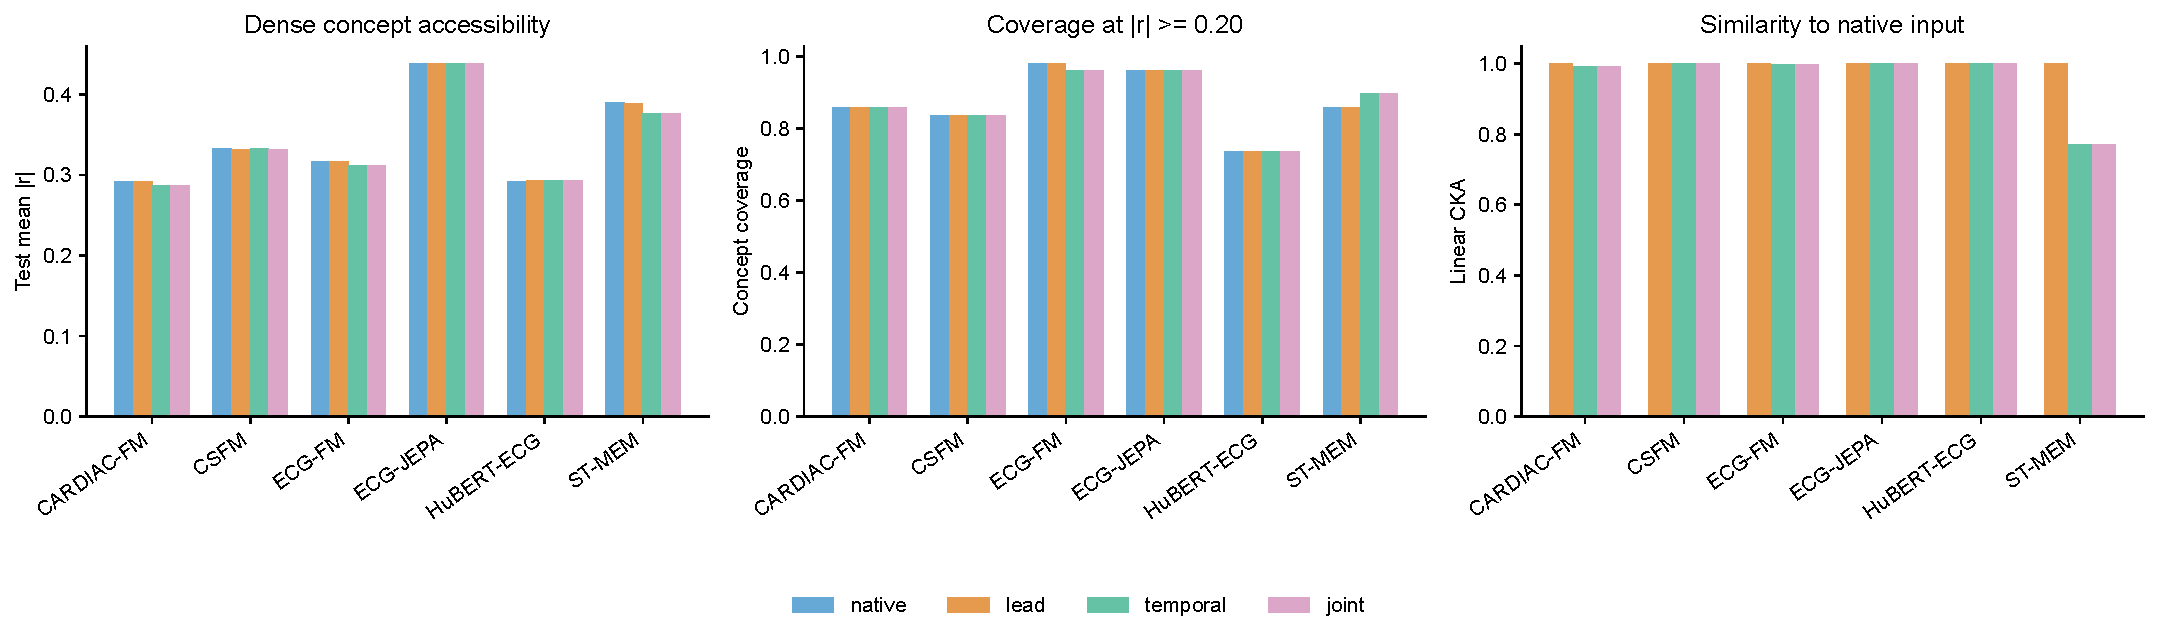
\includegraphics[width=\textwidth]{figures/input_harmonization_final_layer.pdf}
  \caption{Final-layer accessibility under native, lead-harmonized, temporal-harmonized, and jointly harmonized inputs. Left: test mean absolute correlation after training-only coordinate selection. Center: concept coverage at $|r|\geq0.20$. Right: linear CKA between each harmonized representation and its native counterpart.}
  \Description{Three grouped bar charts compare six ECG foundation models under four input protocols. Lead harmonization leaves accessibility and representations nearly unchanged. Temporal and joint harmonization modestly lower accessibility for CARDIAC-FM and ECG-FM and produce the largest representation change for ST-MEM.}
  \label{fig:input-harmonization}
\end{figure*}

Lead harmonization preserves mean $|r|$ within 0.0006 and achieves lead-to-native CKA of at least 0.9999. Temporal harmonization yields changes of $\Delta=-0.0058$ for CARDIAC-FM (95\% CI $[-0.0095,-0.0022]$, $q=0.016$), $\Delta=-0.0048$ for ECG-FM (95\% CI $[-0.0083,-0.0013]$, $q=0.016$), and $\Delta=-0.0131$ for ST-MEM (95\% CI $[-0.0196,-0.0067]$, $q=0.009$). The nearly identical joint and temporal effects identify time-grid and window handling as the source of the measurable changes. ST-MEM's joint CKA of 0.770 reflects the contrast between its native centered 9-second crop and the harmonized complete 10-second record mapped to 2,250 input points.

Model-level coverage is stable after FDR correction (all $q=1.0$), and the six-model ordering by mean accessibility is identical under every protocol (Spearman $\rho=1.0$; Kendall $\tau=1.0$). Coverage ordering is also stable (Spearman $\rho=0.971$ for temporal and joint). ECG-JEPA and HuBERT-ECG mean differences range from $3.5\times10^{-5}$ to $5.7\times10^{-4}$, further demonstrating the close agreement between native and harmonized accessibility profiles.

Overall, the stable ordering across all four input protocols indicates that the observed cross-model differences primarily reflect encoder-representation structure. Lead harmonization has negligible effect, and temporal harmonization preserves the ordering across models. This audit strengthens the attribution of the benchmark profiles to the learned representations.

\section{Validation-Matched SAE--Dense Intervention Selectivity}
\label{app:matched-effect}

The accessibility analyses ask whether a concept can be read from one coordinate. We additionally test whether a sparse coordinate can change a frozen concept readout with less spillover than a native dense coordinate. This is a final-layer, matched-effect comparison over the same 49 waveform concepts. Both methods receive 768 candidate coordinates: the native FM dimensions for Dense and a fixed, target-independent 768-coordinate subset of the $E=8$ dictionary for SAE. For each concept, the top five coordinates and the high-concept centroid are selected using training data only. Intervention doses are then calibrated on validation data to a common achievable target-readout change, capped at $+0.25$ standard deviations, with a minimum feasible change of $0.05$ and interpolation coefficient at most one. Features, centroids, and doses are frozen before patient-disjoint test evaluation.

The SAE arm uses three training seeds and 20 fixed candidate subsets per seed. Primary inference requires a concept to pass the validation effect gate for all three seeds; failed concepts remain in the fixed denominator and are not replaced. The two primary endpoints are cross-family off-target root mean square change and the corresponding wrong-behavior index (WBI), defined as off-target RMS divided by the absolute target effect. Lower values indicate a more selective intervention. Confidence intervals and two-sided tests use 2,000 paired patient-cluster bootstrap draws, followed by Benjamini--Hochberg correction over the preregistered metric families.

\begin{table*}[t]
  \centering
  \caption{Final-layer matched-effect comparison at $k=5$ across the five models satisfying the all-seed validation gate. The eligibility count $n$ requires all three SAE seeds to pass the gate. WBI and deltas are measured on the patient-disjoint test split; negative SAE--Dense deltas favor SAE.}
  \label{tab:matched-effect-dense-sae}
  \begin{tabular}{lrrrrr}
    \toprule
    Model & $n$ & Dense WBI & SAE WBI & $\Delta$ off-target RMS & $\Delta$ WBI \\
    \midrule
    CARDIAC-FM & 5  & 1.614 & 0.971 & $-0.046$ & $-0.643$ \\
    CSFM       & 11 & \textbf{2.134} & 0.944 & $-0.087$ & $-1.189$ \\
    ECG-JEPA   & \textbf{15} & 1.436 & 0.691 & $-0.057$ & $-0.746$ \\
    HuBERT-ECG & 10 & 1.315 & \textbf{1.138} & $\boldsymbol{-0.014}$ & $\boldsymbol{-0.176}$ \\
    ST-MEM     & 10 & 1.678 & 0.736 & $-0.063$ & $-0.942$ \\
    \bottomrule
  \end{tabular}
\end{table*}

\begin{figure*}[t]
  \centering
  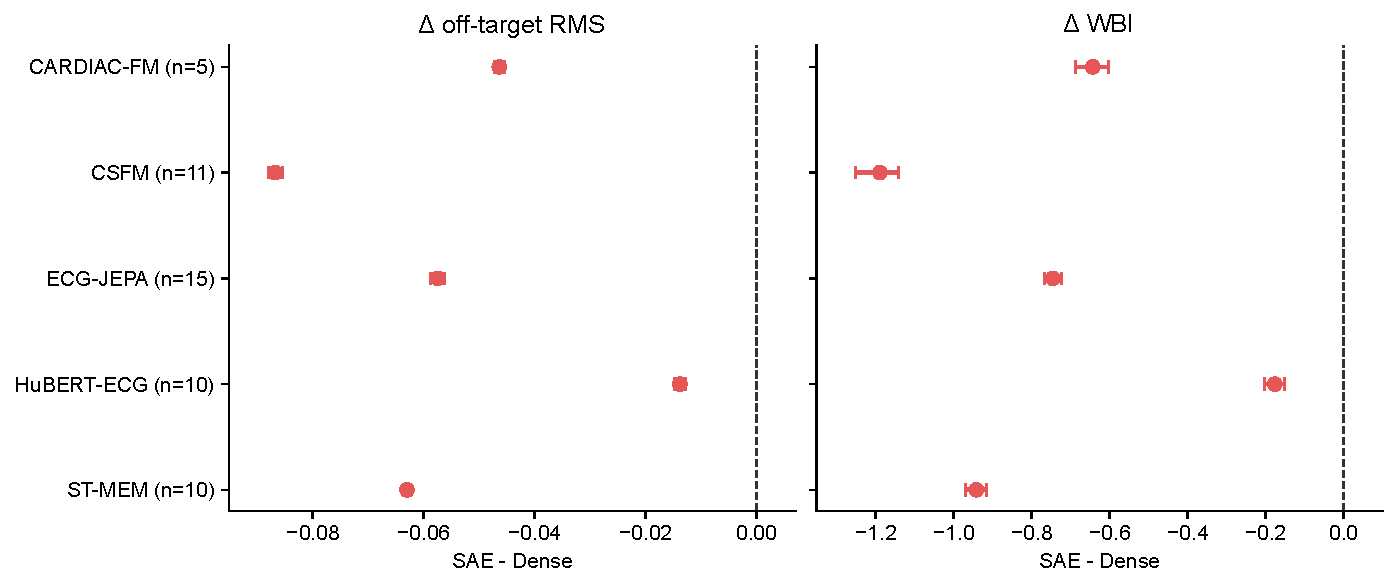
\includegraphics[width=0.9\textwidth]{figures/final_layer_matched_effect_sae_dense_deltas.pdf}
  \caption{SAE--Dense differences in cross-family off-target RMS and WBI with paired patient-cluster 95\% confidence intervals. Negative values favor SAE; model labels give the number of concepts satisfying the strict all-seed gate.}
  \Description{Two forest plots show negative SAE-minus-Dense differences and paired 95 percent confidence intervals for off-target RMS and wrong-behavior index across five models with validation-qualified concepts.}
  \label{fig:matched-effect-sae-dense-deltas}
\end{figure*}

Figure~\ref{fig:matched-effect-sae-dense-deltas} visualizes the paired bootstrap contrasts. All ten 95\% confidence intervals lie entirely below zero, showing consistent SAE reductions in both off-target RMS and WBI across the five models. Off-target RMS differences range from $-0.014$ for HuBERT-ECG to $-0.087$ for CSFM, while WBI differences range from $-0.176$ to $-1.189$ for the same models. CSFM shows the largest reduction on both endpoints, and the favorable direction remains consistent across eligibility sets ranging from 5 to 15 concepts. Across the resulting model--concept evaluations, SAE has a favorable and FDR-significant difference in all 10 model--metric tests ($q\leq .0011$). At a validation-matched frozen readout effect, the selected SAE coordinates consistently produce less cross-family readout spillover than native dense coordinates.
